
\subsection{Epidemiología}

Durante la decada 2000 se ha visto un notable crecimiento de afectados de la enfermedad en la zona de america latina en paises como Paraguay, Brasil, Venezuela Peru. Principalmente en nuestro pais, Paraguay, existen epidemias  de distintos grados de gravedad en cada temporada de verano. Estas epidemias son ocasionadas principalmente por la falta de medidas de prevención y control contra el mosquito transmisor Aedes Aegypti.\\

Si bien es cierto que se realizan campañas contra la enfermedad, los recorridos de fumigacion y limpieza terminan siendo obsoletos ante el no despertar ciudadano frente a la enfermedad. La existencia de grandes cantidades de patios baldíos y terrenos sucios en zonas urbanas dificulta la eliminación del agente transmisor y como consecuencia la enfermedad prevalece y se propaga.\\

La cantidad de afectados por la enfermedad en los ultimos años en todo Paraguay son:
\begin{itemize}
\item 13.766 casos en el año 2010
\item 42.945 casos en el año 2011
\item 2.347 casos en el año 2012
\item 130.155 casos en el año 2013\\
\end{itemize}

El aumento de la población del vector en zonas urbanas del pais, la masiva presencia del virus dengue en los países vecinos, la no colaboración de la poblacion para la eliminacion de criaderos de mosquitos de Aedes aegypti, además de la gran circulación de la poblacion en entre zonas habitadas son alguno de los factores que permiten que la enfermedad siga provocando olas de alerta y riesgo. A estos factores hay qye sumar el factor de la temperatura de nuestro país que es ideal para el desarrollo del agente transmisor.\\


Uno de los objetivos criticos es proveer un sistema de informacion que permita accionar preventivo en zonas de posibles focos de la enfermedad. Cada año en las ultimas 2 decadas se revive la misma situacion, hospitales abarrotados, escases de medicos y medicamentos, situacion de alerta, colapso social ante la epidemia.\\

\subsection{Distribucion Geografica}

El dengue es una enfermedad presente en todo el territorio del Paraguay con fuerte presencia desde hace una decada. Pero la distribucion de la enfermedad no es homogenea sino que se mapea a nivel macro a la distribucion de la poblacion. De ahí que el departamento central es uno de los departamentos con mayor indice de infestación de la enfermedad. En la figura 1 se obserba el resumen de los primeros meses del 2014. Departamentos clasificados segun sean zonas endemicas o no. Los departamentos con mayor densidad poblacional y movimiento de personas son siempre zonas endemicas.\\

Las zonas más afectadas en nuestro país son los departamentos de Central, Amambay e Itapúa. Seguidos de Coordillera, Paraguari y Alto Parana. Otras zonas y departamentos también presentan casos de la enfermedad solo que no son consideradas zonas endemicas o de riesgo. Esta distribución que denota las zonas de mayor riesgo se repite en cada época de flagelo de la enfermedad.\\

A nivel intrinseco en los objetivos de este trabajo está realizar resumenes en mapas similares a los que se muestran en las figuras 1, 2 y 3 pero conteniendo informacion a priori sobre la enfermedad. No señalar las zonas endemicas o no endemicas sino señalar las posibles zonas endémicas o no endémicas según información recolectada sobre la distribución larvaria. Esto permitiría realizar planes de control y prevención de la enfermedad.\\

\begin{figure}
\centering
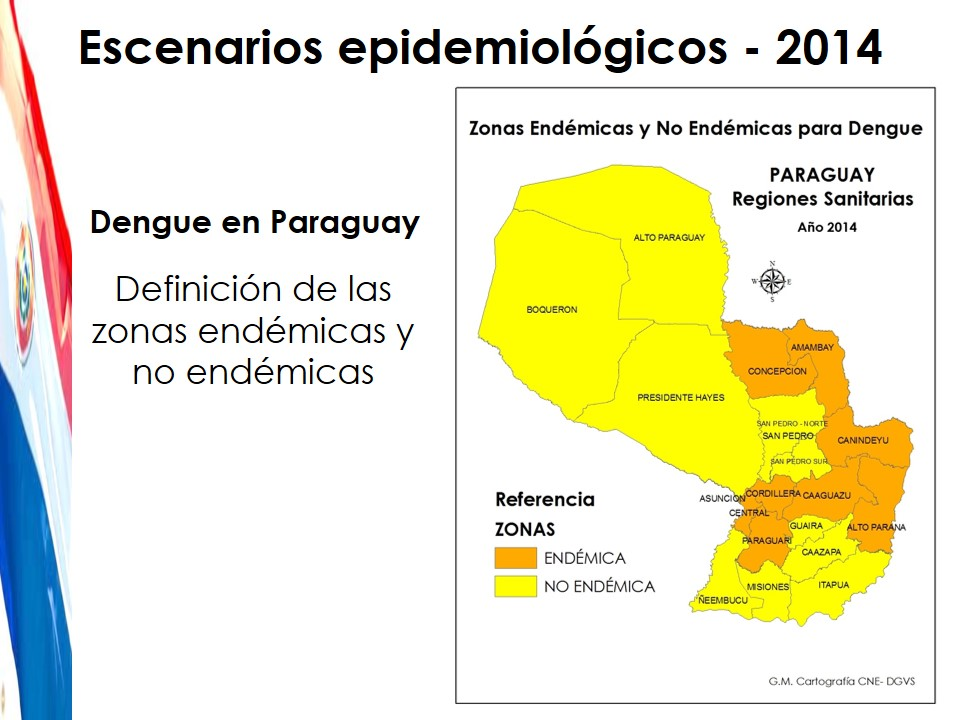
\includegraphics[width=0.8\textwidth]{./graphics/Diapositiva03.JPG}
\caption{\label{fig:mapa1}Zonas endemicas en todo el pais. Anho 2014}
\end{figure}

\begin{figure}
\centering
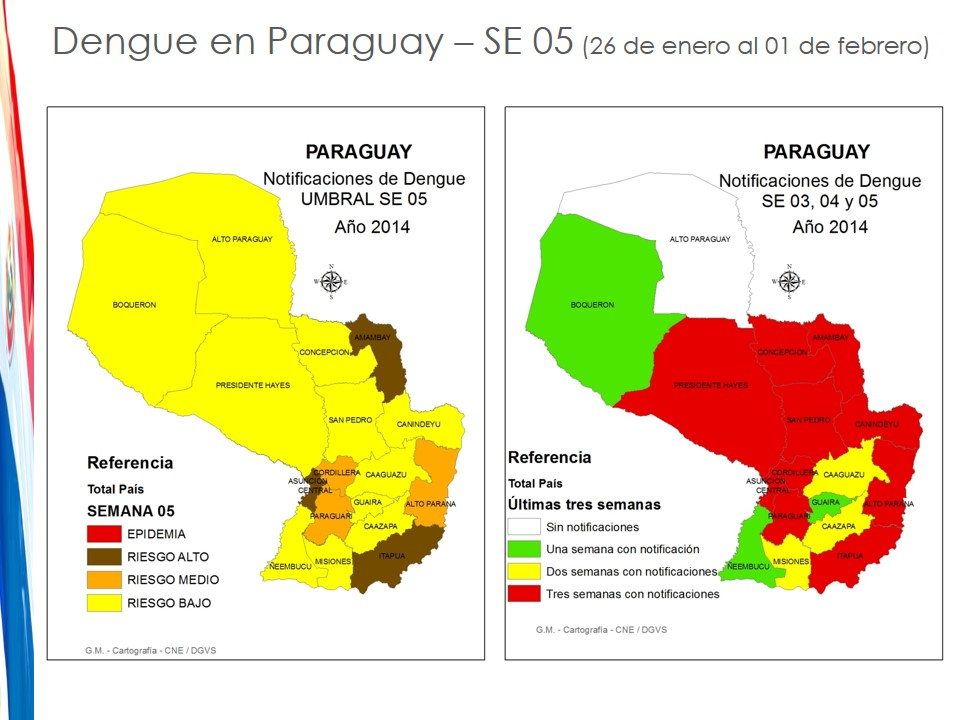
\includegraphics[width=0.8\textwidth]{./graphics/Diapositiva04.JPG}
\caption{\label{fig:mapa2}Mapa de riesgo de la semana epidermiologica 05. Anho 2013 }
\end{figure}

\begin{figure}
\centering
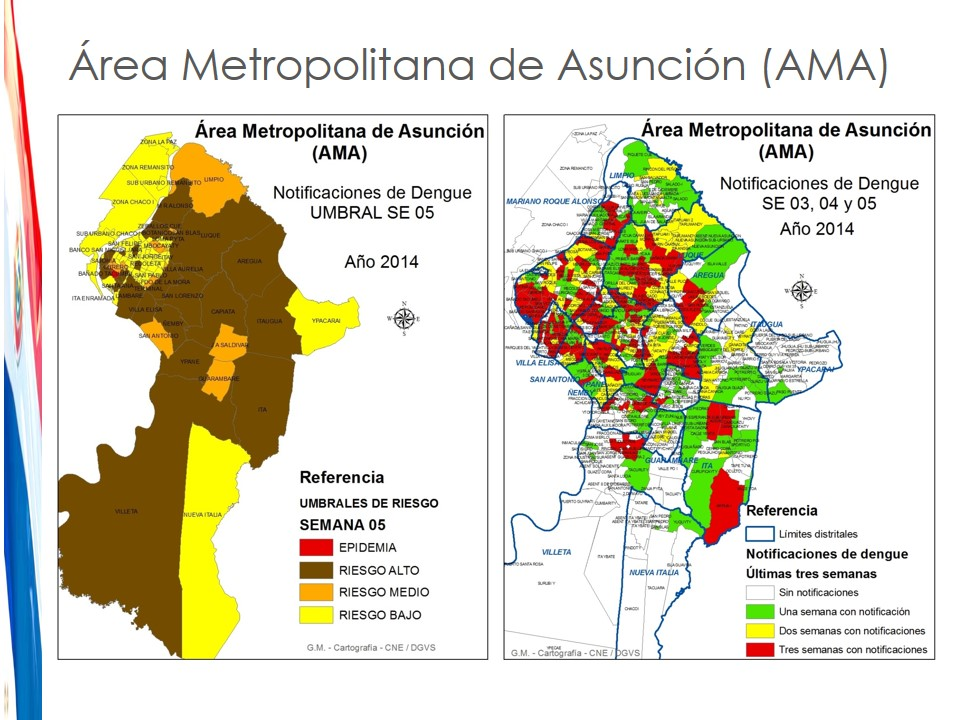
\includegraphics[width=0.8\textwidth]{./graphics/Diapositiva05.JPG}
\caption{\label{fig:mapa3}Mapa del area metropolitana de Asuncion.}
\end{figure}

\subsection{Salud publica}
Cada año el ministerio de salud pública y bienestar social (MSPyBS) en conjunto con otras organizaciones estatales y privadas realiza un plan de de acción en contra de la enfermedad. Un documento detallado presenta el proyecto y los responsables de llevarlo a cabo. El problema de los planes de acción es la dependencia del accionar ciudadano.
Del documento Dengue Plan 12 11 13 del MSPyBS se menciona los objetivos del plan de acción: \\

\textit{"...Los objetivos específicos para cada pilar son los siguientes:\\
\begin{enumerate}
\item Coordinación y Planificación: Fomentar el trabajo intersectorial, el monitoreo y la difusión del plan de acción
\item Vigilancia Entomológica: Vigilar, informar y alertar sobre riesgos ambientales
\item Control Vectorial: Disminuir la población de mosquitos
\item Vigilancia Laboratorial: Garantizar la representatividad de la vigilancia
\item Laboratorio de apoyo en Servicios: Garantizar el acceso a pruebas laboratoriales de diagnóstico
\item Vigilancia Epidemiológica: Aumentar la sensibilidad y oportunidad de la vigilancia
\item Componente Ambiental: Promover intervenciones sobre determinantes de la presencia del mosquito
\item Promoción y Participación Social: Fomentar la movilización social en acciones de control y prevención
\item Comunicación: Informar a la población sobre la problemática del dengue
\item Atención Integral: Asegurar la atención adecuada y oportuna a las personas con síndrome febril agudo con sospecha de dengue..."
\end{enumerate}}

Se concluye de los objetivos la dependencia del accionar de la población. Sin el apoyo de la ciudadanía no es posible controlar el vector ni realizar una vigilancia efectiva . La participación ciudadana tiene que empezar desde el conocimiento de la enfermedad y del vector transmisor. A eso debe sumarse la predisposición para realizar la limpieza del hogar/es propios mediante la eliminación de recipientes que acumulen agua principalmente. El problema es la enorme cantidad de patios baldíos y terrenos desabitados que luego de lluvias terminan siendo sitios propensos para alojar al mosquito.\\


La propuesta realizada en este trabajo tambíén requiere de la participación de la ciudadanía, pero desde un punto de vista distinto ya que el plan de acción será aplicado a las zonas de alto índice de población larval en primer lugar, permitiendo optimizar recursos y fuerza. Requerir de la acción ciudadana luego de que se presenten casos de la enfermedad se torna imposible, el estado de alerta desata preocupación y poco interés en luchar contra la enfermedad. La población en caso de riesgo busca refugiarse del la ola de la enfermedad y aunque existe colaboración para realizar un control sobre el vector el hecho de que ya exista afectados impide lograr una lucha eficiente.
